\documentclass[tikz, border=10pt]{standalone}
\usepackage{pgfplots}
\usepackage{amsmath}
\usetikzlibrary{backgrounds}
\pgfplotsset{compat=1.18}

\begin{document}
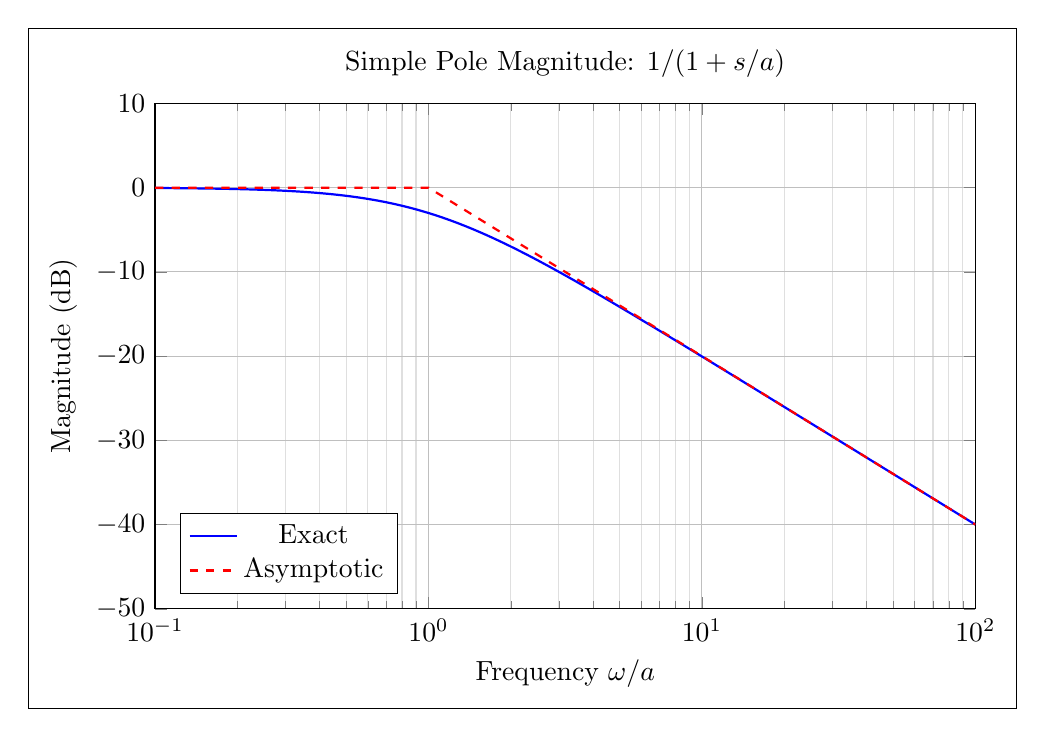
\begin{tikzpicture}[show background rectangle]
    \begin{semilogxaxis}[
        width=12cm, height=8cm,
        title={Simple Pole Magnitude: $1/(1+s/a)$},
        xlabel={Frequency $\omega/a$},
        ylabel={Magnitude (dB)},
        grid=both,
        xmin=0.1, xmax=100,
        ymin=-50, ymax=10,
        minor grid style={gray!25},
        major grid style={gray!50},
        legend pos=south west,
    ]

    % Exact: -20log10(sqrt(1+x^2))
    \addplot[blue, thick, domain=0.1:100, samples=300] {-20*log10(sqrt(1+x^2))};
    \addlegendentry{Exact}

    % Asymptotic: 0 until 1, then -20dB/dec
    \addplot[red, dashed, thick] coordinates {
        (0.1, 0) (1, 0) (100, -40)
    };
    \addlegendentry{Asymptotic}
    
    \end{semilogxaxis}
\end{tikzpicture}
\end{document}
